\documentclass[letterpaper,11pt]{article}


%\usepackage[latin1]{inputenc}
\usepackage[utf8]{inputenc}
\usepackage[spanish,activeacute]{babel}
\usepackage{amssymb}
\usepackage{amsfonts}
\usepackage{hyperref}
\usepackage{amsmath}      % Debe estar despues de babel !!!

\parindent=0cm
\parskip=3mm
\linespread{1.2}

\usepackage[margin=2cm]{geometry}
\usepackage[pdftex]{graphicx} %Para poner gráficas jpg y generar pdf


%\pagestyle{empty}

\begin{document}

\begin{center}
\begin{tabular}{|| c || c ||}
\hline
\hline
		\begin{minipage}{4.5cm}
			\begin{center} 
				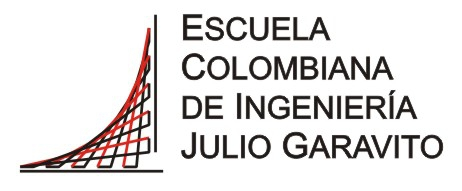
\includegraphics[width=120pt]{escuela.jpg}\\
			\end{center}
		\end{minipage}
	&
		\begin{minipage}{11cm}
			\begin{center}
			\vspace{.1cm}
				\Large{Coordinación de proyectos de grado}\\
				\Large{Formulación de Proyecto de Grado}\\
				2012 - 1
			\vspace{.1cm}
			\end{center}
		\end{minipage}\\
\hline
\end{tabular}
\end{center}

\section{Información general del proyecto de grado}

\begin{center}
\begin{tabular}{| c | c |}
\hline
\hline
		\begin{minipage}{4.5cm}
			\begin{center}
			\vspace{.1cm}
				Nombre\\
			\vspace{.1cm}
			\end{center}
		\end{minipage}
	&
		\begin{minipage}{11cm}
			\begin{center}
			\vspace{.1cm}
				MAEOCS\\ (Mobile Aplication for Easy Orientation in 
				Confined Spaces)
			\vspace{.1cm}
			\end{center}
		\end{minipage}\\
\hline
		\begin{minipage}{4.5cm}
			\begin{center}
			\vspace{.1cm} 
				Director\\
			\vspace{.1cm}
			\end{center}
		\end{minipage}
	&
		\begin{minipage}{10cm}
			\begin{center}
			\vspace{.1cm}
				Rodrigo López\\
			\vspace{.1cm}
			\end{center}
		\end{minipage}\\
\hline
		\begin{minipage}{4.5cm}
			\begin{center}
			\vspace{.1cm} 
				Equipo de estudiantes\\
			\vspace{.1cm}
			\end{center}
		\end{minipage}
	&
		\begin{minipage}{10cm}
			\begin{center}
			\vspace{.1cm} 
				Carlos Gaitán y 
				Edward Jiménez\\
			\vspace{.1cm} 
			\end{center}
		\end{minipage}\\
\hline
		\begin{minipage}{4.5cm}
			\begin{center}
			\vspace{.1cm} 
				Grupo de investigación\\
			\vspace{.1cm}
			\end{center}
		\end{minipage}
	&
		\begin{minipage}{10cm}
			\begin{center}
			\vspace{.1cm}
				CTG Informática
			\vspace{.1cm}
			\end{center}
		\end{minipage}\\
\hline
		\begin{minipage}{4.5cm}
			\begin{center}
			\vspace{.1cm} 
				Línea de investigación\\
			\vspace{.1cm}
			\end{center}
		\end{minipage}
	&
		\begin{minipage}{10cm}
			\begin{center}
			\vspace{.1cm}
				Informática e Infraestructura\\
			\vspace{.1cm}
			\end{center}
		\end{minipage}\\
\hline
		\begin{minipage}{4.5cm}
			\begin{center}
			\vspace{.1cm} 
				Proyecto de investigación al que pertenece\\
			\vspace{.1cm}
			\end{center}
		\end{minipage}
	&
		\begin{minipage}{10cm}
			\begin{center}
			\vspace{.1cm}
				Informática e Infraestructura\\
			\vspace{.1cm}
			\end{center}
		\end{minipage}\\
\hline
		\begin{minipage}{4.5cm}
			\begin{center}
			\vspace{.1cm} 
				Duración (Meses)\\
			\vspace{.1cm}
			\end{center}
		\end{minipage}
	&
		\begin{minipage}{10cm}
			\begin{center}
			\vspace{.1cm}
				12\\
			\vspace{.1cm}
			\end{center}
		\end{minipage}\\
\hline
\end{tabular}
\end{center}

\section{Resumen ejecutivo}

	El proyecto se centra en desarrollar una aplicación móvil  que permita una fácil orientación 
	dentro de una instalación pública o privada sin necesidad de 
	tecnologías costosas; se plantea una aplicación sencilla de 
	manipular que permita a las personas desde sus celulares hacer 
	diferentes preguntas sobre su localización y que les muestre el 
	camino que pueden tomar para llegar a su lugar de destino, dando 
	una posible solución a los problemas de ubicación en instalaciones dentro de un 
	espacio cerrado.

\section{Descripción del proyecto}
	
	\subsection{Planteamiento del problema.}
	
	Hoy en día es fácil evidenciar cómo los planteles públicos y 
	privados van en crecimiento ampliando sus zonas e incluso 
	dispersándolas en diferentes puntos de un mismo sector; por ello, 
	las personas que son nuevas en dichos planteles, poseen mala 
	memoria o problemas de orientación se ven afectadas perdiéndose y 
	quedándose varios minutos frente a un mapa en el cual no pueden 
	ubicarse.

	Es útil plantear una solución que permita orientar a las 
	personas en planteles de tamaños considerables; 
	claro está de la manera más sencilla y con la menor cantidad de 
	tecnología posible para que sea accesible a  personas de 
	todas las edades.
		
	\subsection{Justificación}
	
	La ubicación en instalaciones de grandes tamaños es un grave problema 
	para las instituciones que siempre buscan la comodidad de 
	las personas que se mueven dentro de ellas. La fácil 
	orientación puede llegar a ser un factor decisivo para los clientes 
	de dichas instituciones cuando hablamos de visitas, compras o 
	ventas; por ello se plantea el desarrollo de una aplicación para 
	dispositivos móviles fácil de manejar, que dé solución a este 
	problema. La aplicación facilitará la ubicación de un cliente, le permitirá 
	escoger su destino, se encargará de calcular las 
	rutas posibles y le ofrecerá al usuario la más conveniente. 
	
	\subsection{Marco teórico y estado del arte}
	
	El tema de ubicación es un problema de la vida cotidiana para 
	la humanidad el cual ha venido siendo tratado desde la antigüedad 
	con mapas y brújulas e incluso la naturaleza. A este respecto,
	la actualidad lo primero que llama la atención son los sistemas 
	avanzados como los GPS, fotos de mapas con satélites y aplicaciones 
	con	mapas geográficos. En el caso de los mapas no se puede pasar por 
	alto a \href{http://earth.google.es}{Google Earth} una aplicación 
	que	permite observar fotos que fueron tomadas desde satélites como 
	mapas e incluso buscar diferentes lugares señalados en éstas.
	
	Si pensamos en conocer la ubicación de ciertos lugares los mapas son
	una buena herramienta pero si lo que se quiere es conocer la 
	posición exacta, dicha herramienta puede llegar a ser confusa e 
	insuficiente dependiendo de qué tan escalado o específico sea el 
	mapa; por ello mismo nació la tecnología del GPS (Global Positioning 
	System) la cual nos permite conocer nuestra posición exacta en un 
	mapa de	manera precisa y constante.
	
	Aun cuando se puede saber la posición exacta en un mapa desde algún 
	tipo de tecnología, pocas son las aplicaciones que existen y grande 
	es el problema cuando lo que se trata de conocer es el camino más 
	corto entre donde se encuentra una persona y el lugar al que ésta
	quiere ir. Para problemas como lo es el de hallar el camino más 
	corto entre un punto y sus múltiples opciones se han planteado 
	varias soluciones desde el punto de vista algorítmico; algunas de 
	estas soluciones son:
	
	\begin{itemize}
		\item Algoritmo de Dijsktra, resuelve problemas del tipo ``camino 
		más corto'' desde un vértice origen a los demás vértices del 
		grafo.

		\item Algoritmo de Floyd - Warshall, resuelve problemas del tipo 
		``camino más corto'' para todos los vértices.

		\item Algoritmo de Johnson, resuelve problemas del tipo ``camino 
		más corto'' para todos los vértices en grafos de baja densidad.

	\end{itemize}

    Hoy en día con el crecimiento de los videojuegos y gracias al código libre 
    que podemos encontrar fácilmente en internet para su creación (en 
    especial los RPG\footnote{Role-Playing Game}), podemos analizar y 
    visualizar las diferentes técnicas que usan para crear e 
    interpretar los mapas de los diferentes mundos, una de ellas es el 
    mallado de imágenes; poniendo una imagen como fondo se crea una 
    malla sobre está y los edificios, puntos importantes y caminos se 
    definen como objetos que se colocan en cada celda y así se va 
    creando un mapa virtual fácil de reconocer para la aplicación. 
	
	\subsection{Objetivos generales y específicos}
	
	A través de una aplicación fácil de manejar, facilitar la 
	orientación	dentro de una institución a través de un mapa de la 
	misma. La aplicación podrá ser accedida desde cualquier dispositivo 
	móvil con sistema operativo 
	\href{http://www.android.com/about/}{Android} y permitirá al 
	usuario, desde su 
	ubicación, escoger su destino y guiarle hasta él a través de
	algoritmos de búsqueda que por debajo de la aplicación calcularán la 
	ruta más corta para luego ser descrita en la interfaz de la 
	aplicación donde el usuario podrá verla.

	Para la creación del mapa que se cargará en la aplicación móvil será 
	necesario un software que permita importar un plano y, a partir de él, crear un mapa
	especial permitiendo ubicar dentro del mismo
	los caminos, puntos importantes, edificios, los posibles destinos, 
	etc.
	
	\subsection{Alcance del proyecto}
	
        Con este proyecto se pretende obtener dos productos concretos:

		Una aplicación para definición de mapas. Esta aplicación permite de manera sencilla señalizar 
		diferentes caminos y lugares en un mapa para calcular los caminos 
		óptimos entre todos los puntos y al final generar un archivo con 
		el mapa y todo lo que se necesite para poder orientar a una persona.
		Por ejemplo, importar el mapa del centro comercial Santa Fe y ubicar 
		en éste las tiendas, baños, ascensores, escaleras, entradas y puntos 
		de atención de manera sencilla.

	\subsection{Metodología propuesta}
	
	\begin{itemize}
		\item 	El proyecto será dividido en dos fases que corresponden 
		al alcance del proyecto y cada fase a su vez será dividida en 
		actividades que serán publicadas para que los miembros del 
		grupo las realicen en el tiempo acordado.

		\item Se usará \LaTeX como formateador para la creación de 
		documentos.

		\item \href{http://maeocs.pbworks.com}{PBWorks} será la página 
		central para que todos los miembros 
		publiquen y consulten los diferentes entregables, fechas y 
		materiales del proyecto.
		
		\item Aparte de las reuniones semanales establecidas por la 
		escuela se publicarán comentarios y se mantendrán conversaciones 
		activas	a través del PBWorks para mantener una comunicación 
		fluida entre los miembros.
	\end{itemize}
	
	\subsection{Área de aplicación del producto resultado del proyecto}
	
        Aplicaciones novedosas de la tecnología móvil para asistir a las 
        personas.
	
	\subsection{Resultados esperados}
	
	\begin{itemize}
		\item La aplicación creadora de mapas en 2D terminada.

		\item La aplicación móvil terminada para dispositivos con
		sistema operativo Android terminada.

		\item Documento guía para la creación e interacción de 
		aplicaciones para dispositivos con sistema operativo Android.

	\end{itemize}

	\subsection{Usuarios potenciales directos e indirectos de los 
	resultados de la  investigación}
	
	\begin{itemize}
		\item Instituciones con amplias instalaciones.

		\item Centros Comerciales.

		\item Instituciones con una mala/dispersa organización de sus 
		instalaciones.

		\item Personas con problemas de orientación o memoria.
	\end{itemize}

	\subsection{Cronograma}
			
	\begin{itemize}
		\item Fecha de entrega Martes 21/02 - 28/02: 
		
		Adquirir requerimientos, hacer análisis y crear un diseño 
		básico de la aplicación. 
		
		Entregable Principal: Diagrama de Clases.

		\item Fecha de entrega Martes 06/03: 
		
		Creación del prototipo y discusión sobre la creación de la 
		grilla para el mapa.
		
		Entregable Principal: Prototipo de la aplicación.

		\item Fecha de entrega Martes 13/03: 
		
		Implementar la grilla para los mapas y discusión del 
		método para arrastrar los ítem de un panel a la grilla.
		
		Entregable Principal: Esqueleto de la aplicación e 
		implementación de la grilla en el.
		
		\item Fecha de entrega Martes 20/03 - 27/03: 
		
		Implementar el arrastre de objetos a la grilla para los mapas 
		y discusión del	algoritmo para resolver los posibles caminos.
		
		Entregable Principal: Implementación del arrastre de objetos a 
		la grilla en el esqueleto de la aplicación.
		
		\item Fecha de entrega Martes 10/04 - 17/04: 
		
		Implementación del método para resolver los posibles caminos del 
		mapa y últimos arreglos a la interfaz de la aplicación.
		
		Entregable Principal: Aplicación generadora de mapas para el el 
		aplicativo en Android para dispositivos móviles.
				
	\end{itemize}
	
	\subsection{Herramientas de software utilizadas}

	Usaremos un ambiente de Elcipse con plugins especializados para 
	programar aplicaciones que funcionen sobre Android.

	PBWorks es una herramienta que usamos como página de control para los 
	entregables y consultas del proyecto.
	
	\subsection{Criterios de terminación del trabajo}
	
	\begin{itemize}
		\item Las aplicaciones propuestas deben estar terminadas tanto 
		en su parte funcional como en su documentación.

		\item Los documentos de la investigación deben estar terminados 
		cumpliendo con los requisitos y estándares acordados.
	\end{itemize}
	
	\subsection{Evaluadores}
	
	Ing. Héctor Fabio Cadavid Rengifo
	
	Ing. Juan Carlos Marino 	
	
	\subsection{Bibliografía}
	
	\begin{thebibliography}{9}
	
		\bibitem{Android in Action}
		W. Frank Ableson, Robi Sen and Chris King, \emph{Android in Action
		}, MANNING, Greenwich, 2011.
		
		\bibitem{Tiled} T. Lindeijer, \emph{Tiled Map Editor},  
		preprint (2011), available at 
		\url{http://www.mapeditor.org/}.
		
		\bibitem{Mappy} \emph{Mappy Editor},  
		available at 
		\url{http://tilemap.co.uk/mappy.php}.

	\end{thebibliography}

\end{document}
